\subsection{DATOS}
Amplificador Operacional LM324.

$Vcc = 10V$  $Vss = -10V$

D1 = D2 = 1N4148

R1 = R3 = R4 = $10K\Omega$ $1\%$ y $R2 = 5K\Omega$ $1\%$

\begin{center}
	\resizebox{14cm}{!}{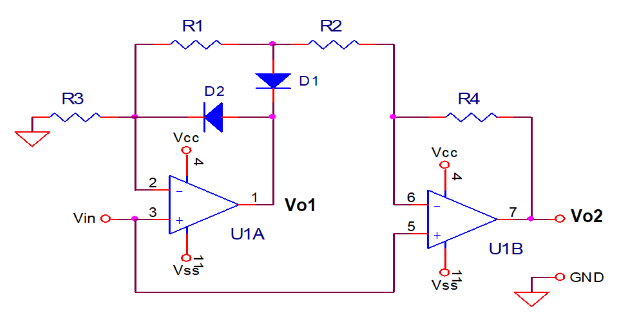
\includegraphics{Imagenes/CIII.png}} \\
	\stepcounter{figure}
	\begin{center}
    	\begin{small}
        \textit{Fig.\thefigure \ - \ 	Circuito III: Rectificador de precisión.}
		\end{small}
    \end{center}
\end{center}

\subsection{PARÁMETROS/RELACIONES A ANALIZAR:}

\noindent \textbf{ANALÍTICO:}
\begin{enumerate}[3.1]
    \item $V_{o1} = f(V_{in}), V_{o2} = f(V_{in})$; con $0V < V_{in}$ (Ignorar Rd del diodo)
    \item $V_{o1} = f(V_{in}), V_{o2} = f(V_{in})$; con $V_{in} > 0V$ (Ignorar Rd del diodo)\end{enumerate}

\subsection{MEDICIÓN - SIMULACIÓN:}
\begin{enumerate}[3.3]
    \item Gráfico Entrada/Salida: $V_{o1}=f(V_{in})$\hspace{0.25cm} y \hspace{0.25cm} $V_{o2} = f(V_{in})$ \hspace{0.25cm}$Vss < V_{1} < Vcc$
\end{enumerate}
